\chapter{GNN \& GCN}

Negli ultimi anni, l’apprendimento automatico ha compiuto notevoli progressi, in particolare grazie ai modelli profondi applicati all’analisi di dati strutturati come sequenze (con RNN e Transformer) o immagini (mediante le reti convoluzionali, le celebri CNN). Tuttavia, molti dati del mondo reale non seguono strutture regolari come quelle di una griglia o di una sequenza ordinata. In questi casi, i grafi offrono una rappresentazione ben più adatta: strutture composte da nodi (gli elementi) e archi (le connessioni tra essi), in grado di modellare relazioni complesse come quelle presenti nei social network, nelle molecole, nei testi, nelle immagini o nei sistemi biologici e di raccomandazione. Questo capitolo è dedicato al Graph Machine Learning, ovvero all'applicazione del deep learning ai dati rappresentati come grafi. Analizzeremo le Graph Neural Networks (GNN), approfondendo le ragioni della loro efficacia e le sfide che pongono. Esamineremo le principali famiglie di modelli, i diversi tipi di problemi che possono risolvere (a livello di nodo, di collegamento o dell’intero grafo) e le tecniche per rappresentare e manipolare i dati strutturati all’interno di una rete neurale. In particolare, ci soffermeremo sulle Graph Convolutional Networks (GCN), che estendono il concetto di convoluzione dal dominio delle immagini a quello dei grafi. Approfondiremo anche modelli più recenti e avanzati, come le Graph Attention Networks (GAT), GraphSAGE e le Graph Isomorphism Networks (GIN). Lungo il percorso introdurremo concetti fondamentali come il \textit{message passing} (lo scambio di informazioni tra nodi), l’equivarianza rispetto alle permutazioni, la scalabilità e la necessità di rappresentare in modo coerente non solo i nodi e gli archi, ma anche il contesto complessivo. L’obiettivo è fornire una base teorica e pratica solida per comprendere come applicare il deep learning anche su dati complessi e connessi come quelli rappresentati dai grafi, aprendo la strada a nuove soluzioni per problemi reali sempre più articolati.

\section{Grafi}

Un \textbf{grafo} è una struttura estremamente flessibile per rappresentare informazioni interconnesse. È composto da elementi chiamati \textit{nodi}, connessi tra loro mediante \textit{archi} (o \textit{spigoli}). A differenza di una lista o di una sequenza, un grafo non presenta un inizio o una fine ben definiti, ed è quindi ideale per descrivere dati complessi che non seguono un ordine lineare. Gli archi possono essere unidirezionali (come nel caso dei follower su Twitter) o bidirezionali (come le amicizie su Facebook), determinando la distinzione tra grafi orientati e non orientati.
\begin{figure}
    \centering
    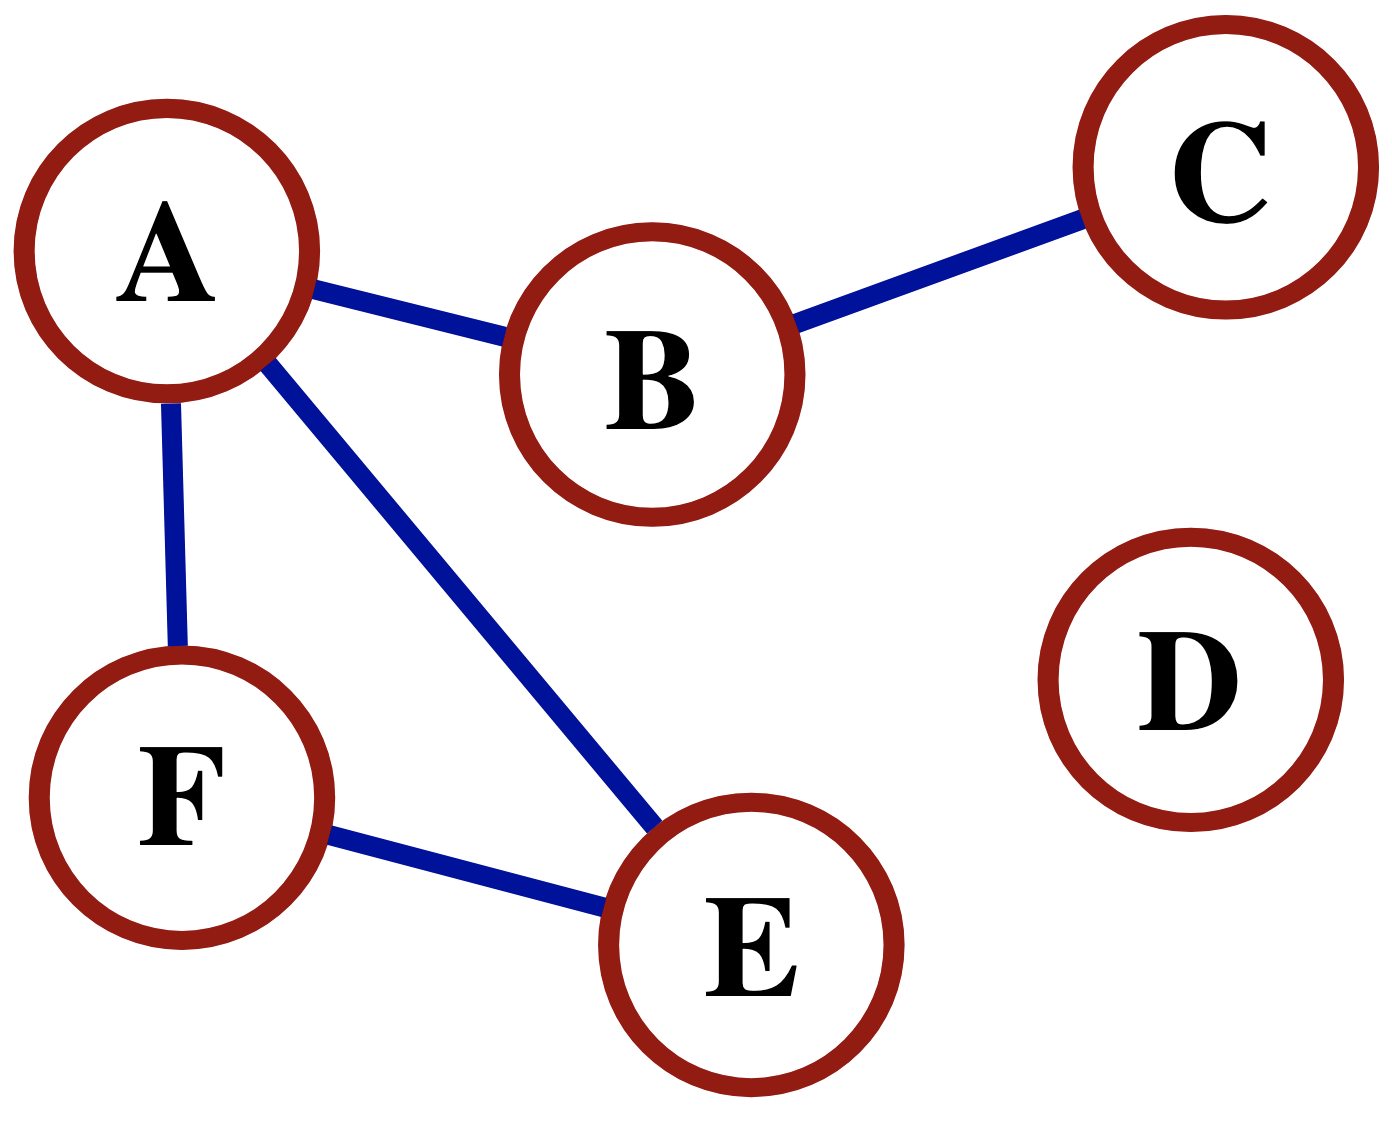
\includegraphics[width=0.45\textwidth]{figure/Graph.png}
    \caption{Esempio di grafo non orientato composto da 6 nodi e 5 archi. Se fosse orientato, gli archi avrebbero delle frecce che ne indicherebbero la direzione.}
    \label{fig:enter-label}
\end{figure}
Ogni componente del grafo può possedere attributi. I nodi, ad esempio, possono essere caratterizzati dalla loro identità o dal numero di connessioni (\textit{grado}), mentre gli archi possono avere un \textit{peso} che quantifica la forza della connessione. Talvolta, si introduce anche un \textit{nodo centrale} (o \textit{master node}) che sintetizza informazioni globali sul grafo, come il numero totale di nodi, archi o la lunghezza massima di un percorso.

\subsection{Immagini come grafi}

Sebbene le immagini siano solitamente rappresentate come matrici di pixel, esse possono essere descritte anche tramite grafi a struttura regolare. In questo contesto, ogni pixel corrisponde a un nodo, collegato ai pixel adiacenti. Un pixel interno ha otto vicini: sopra, sotto, destra, sinistra e lungo le diagonali. L'informazione contenuta in ciascun nodo è il vettore RGB (rosso, verde, blu) del pixel. Per rappresentare le connessioni tra i nodi si utilizza la \textit{matrice di adiacenza}, una struttura che indica quali nodi sono connessi, facilitando così le operazioni computazionali sul grafo.

\begin{figure}
    \centering
    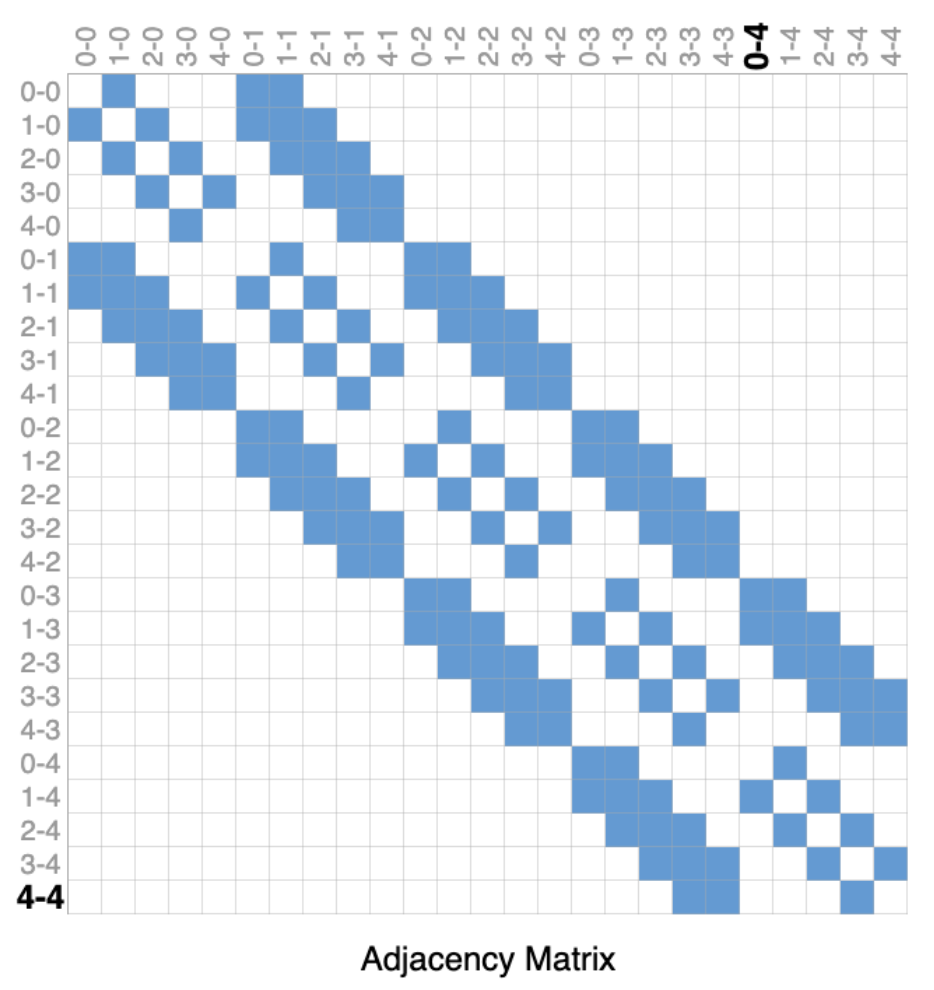
\includegraphics[width=0.5\textwidth]{figure/AdjacencyMatrix}
    \caption{Matrice di adiacenza per un'immagine $5\times5$ raffigurante una faccina sorridente. I nodi (pixel) sono connessi se condividono un lato.}
    \label{fig:adjMatrix}
\end{figure}

\subsection{Testi come grafi}

Nonostante sia possibile modellare testi e immagini come grafi, ciò non è comune in quanto tali dati possiedono strutture regolari. Nei testi, per esempio, ogni parola è connessa solo a quella precedente e a quella successiva, producendo matrici di adiacenza fortemente strutturate, spesso con una diagonale che riflette questa linearità.
\begin{figure}
    \centering
    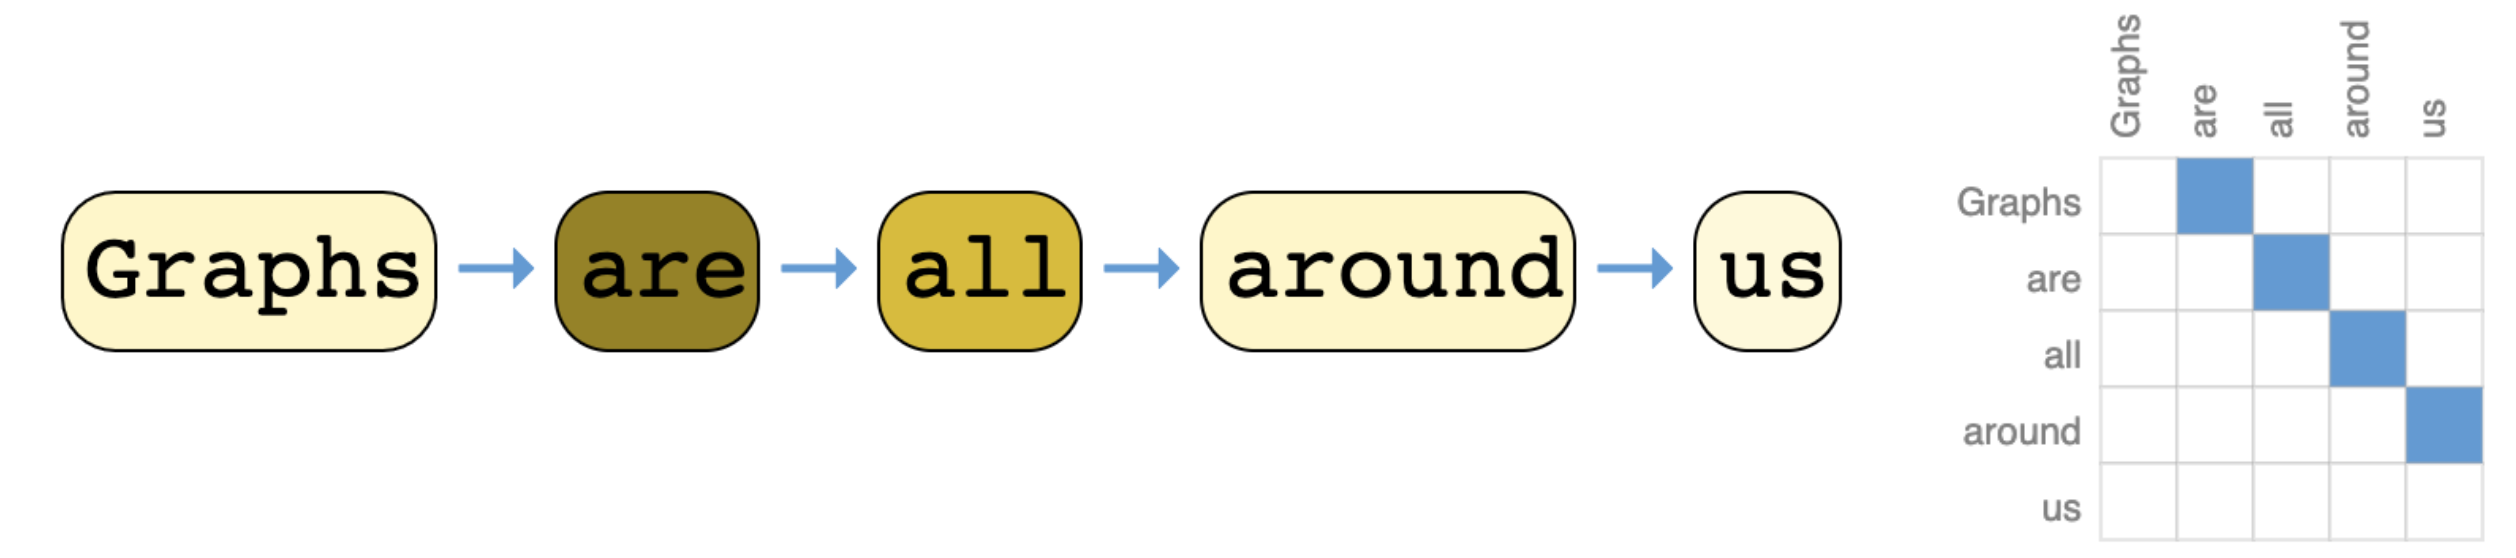
\includegraphics[width=\textwidth]{figure/TextGraph.png}
    \caption{Matrice di adiacenza di un testo: ogni parola è connessa alla precedente e alla successiva, dando origine a una struttura diagonale.}
    \label{fig:textGraph}
\end{figure}
L’uso dei grafi diventa veramente vantaggioso quando ci si confronta con dati irregolari e relazioni complesse non lineari.

\subsection{Graph-level task}

In un \textbf{Graph-level task}, l’obiettivo è predire una proprietà che riguarda l’intero grafo. Un caso esemplare è l’analisi di molecole: modellandole come grafi, si può cercare di predire l’odore, la tossicità, o il recettore con cui si legheranno. Questo tipo di task è analogo a quello della classificazione di immagini (es. dataset MNIST o CIFAR), in cui si assegna un’etichetta all’intera immagine. Anche nel NLP troviamo un parallelo: la \textit{sentiment analysis}, che determina il tono emotivo di un intero testo.

\subsection{Node-level task}

Nei \textbf{Node-level task}, l’obiettivo è classificare ciascun nodo individualmente. Un esempio classico è il \textit{Zachary’s Karate Club}, un dataset che rappresenta un social network diviso in due fazioni a seguito di un conflitto tra due leader. Il compito consiste nel prevedere a quale fazione appartiene ciascun membro.
\begin{figure}
    \centering
    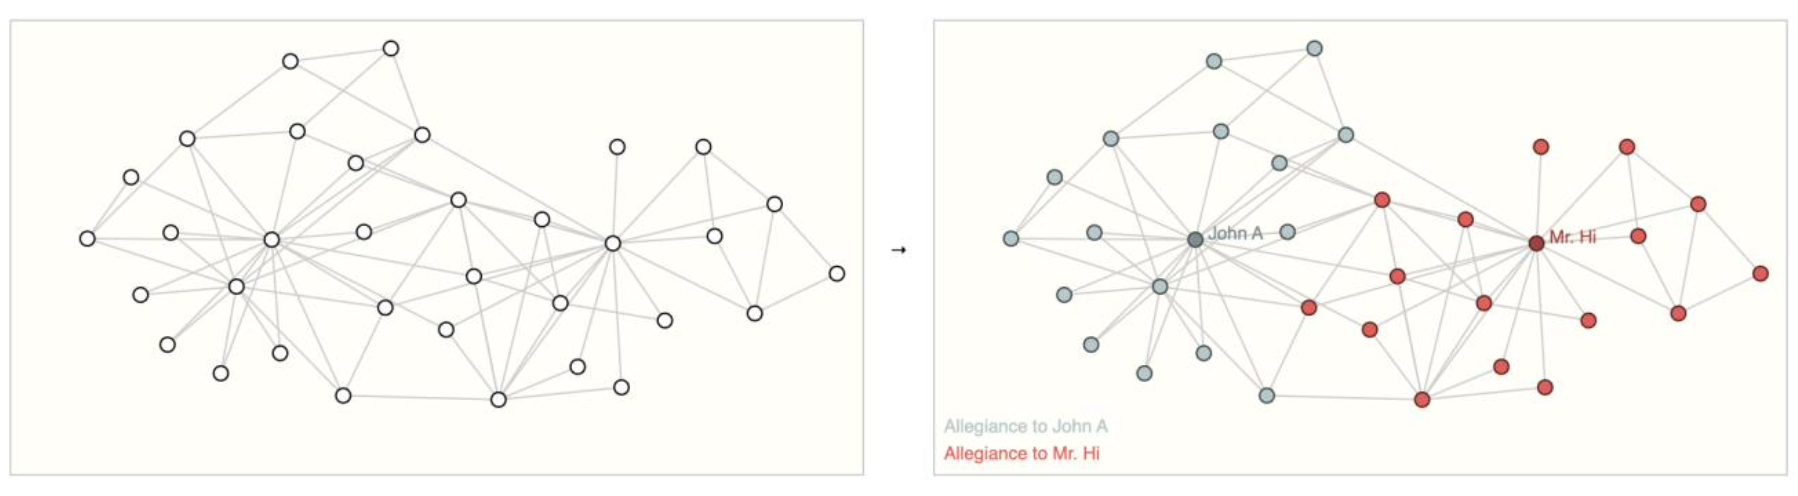
\includegraphics[width=\textwidth]{figure/ZachsKarateClubProblem.png}
    \caption{Zachary’s Karate Club: a sinistra, la rete prima della divisione; a destra, i due gruppi dopo lo scisma.}
    \label{fig:ZKCProblem}
\end{figure}
Questo problema è analogo alla segmentazione nelle immagini, in cui ogni pixel viene etichettato. Nel NLP, un compito simile è il \textit{part-of-speech tagging}, dove si assegna a ogni parola una categoria grammaticale.

\subsection{Edge-level task}

Un ulteriore tipo di problema è l’\textbf{Edge-level task}, che riguarda la previsione delle relazioni tra coppie di nodi. Un esempio si trova nella comprensione di scene: una rete neurale può essere impiegata non solo per identificare oggetti, ma anche per determinare le relazioni tra essi (es. "il cane è sopra il tappeto"). In questi compiti si costruisce spesso un grafo completamente connesso, per esplorare il maggior numero possibile di interazioni tra nodi e migliorare la comprensione complessiva della struttura.

\section{Computazione sui grafi}

Come abbiamo visto, i grafi sono modelli estremamente flessibili, ma questa flessibilità implica l’assenza di una struttura fissa. Per esempio, nel compito di prevedere la tossicità di una molecola in base alla sua struttura, le molecole in esame possono variare per numero e tipo di atomi, nonché per le caratteristiche dei legami chimici. Rendere questi grafi computabili richiede quindi una rappresentazione adatta al compito. Quando si usano grafi in \textit{machine learning}, una semplice permutazione dei nodi può produrre matrici di adiacenza diverse pur partendo dallo stesso grafo. Questo rende evidente che non esiste un’unica rappresentazione “corretta”, e il modello deve essere progettato per essere invariante rispetto a queste permutazioni.

\subsection{Ordine dei nodi}

Convertire un grafo in un vettore richiede necessariamente un ordinamento dei nodi. Tuttavia, lo stesso grafo può essere rappresentato in più modi equivalenti. Per questo, un buon algoritmo deve essere \textbf{invariante rispetto all’ordine dei nodi}: qualsiasi permutazione non dovrebbe alterare l’output del modello.
\begin{figure}
    \centering
    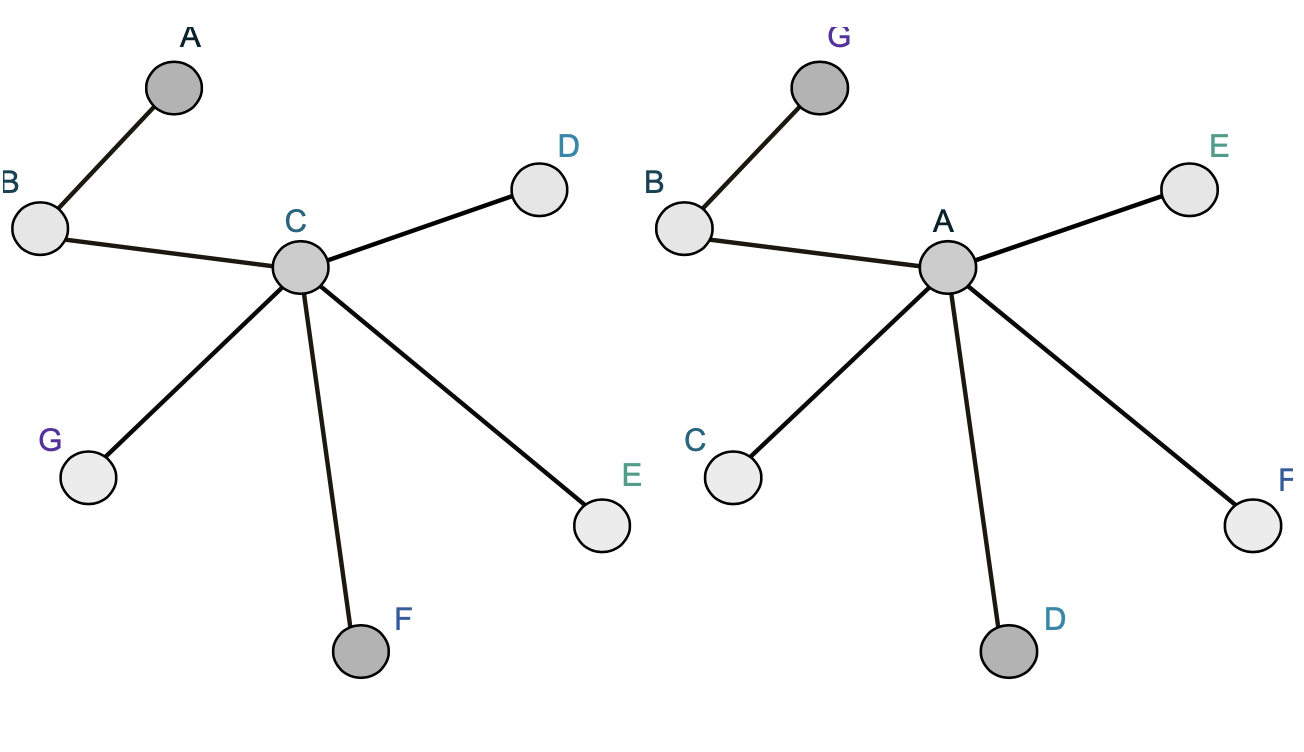
\includegraphics[width=0.8\textwidth]{figure/OrderNode}
    \caption{Due rappresentazioni diverse di un alfabeto attraverso un grafo. Sebbene l’ordine dei nodi sia differente, il significato sottostante è identico.}
    \label{fig:ordNode}
\end{figure}

\subsection{Scalabilità}

I grafi possono raggiungere dimensioni enormi. Basti pensare a social network come Facebook o Twitter, che contano oltre un miliardo di utenti. In questi casi, ogni nodo può avere attributi complessi, e l’insieme delle connessioni forma strutture molto ampie. Fortunatamente, i grafi reali tendono a essere \textit{sparsi}, cioè ogni nodo è connesso solo a una piccola porzione degli altri.

\subsection{Rappresentazione dei grafi}

I grafi possono essere rappresentati in diverse modalità, ma una delle più efficienti in termini di spazio e adatta alla rappresentazione di matrici sparse è la lista di adiacenza (Figura~\ref{fig:GraphComp}). In questo approccio, la connettività tra i nodi viene descritta tramite delle tuple, ciascuna posta nella posizione corrispondente al nodo sorgente all'interno della lista. Questo consente di evitare la computazione e la memorizzazione di porzioni disconnesse del grafo, ipotizzando che il numero di archi sia sensibilmente inferiore al quadrato del numero di nodi (cioè, che la matrice di adiacenza sia sparsa). È importante sottolineare che la rappresentazione mostrata in figura utilizza valori scalari per gli attributi dei nodi, degli archi e del contesto globale, ma nella pratica i modelli GNN operano generalmente con vettori di caratteristiche. Pertanto, anziché avere un tensore dei nodi di dimensione $[\textit{n nodes}]$, avremo un tensore di forma $[\textit{n nodes}, \textit{node dim}]$, e analogamente per archi e attributi globali.

\begin{figure}
    \centering
    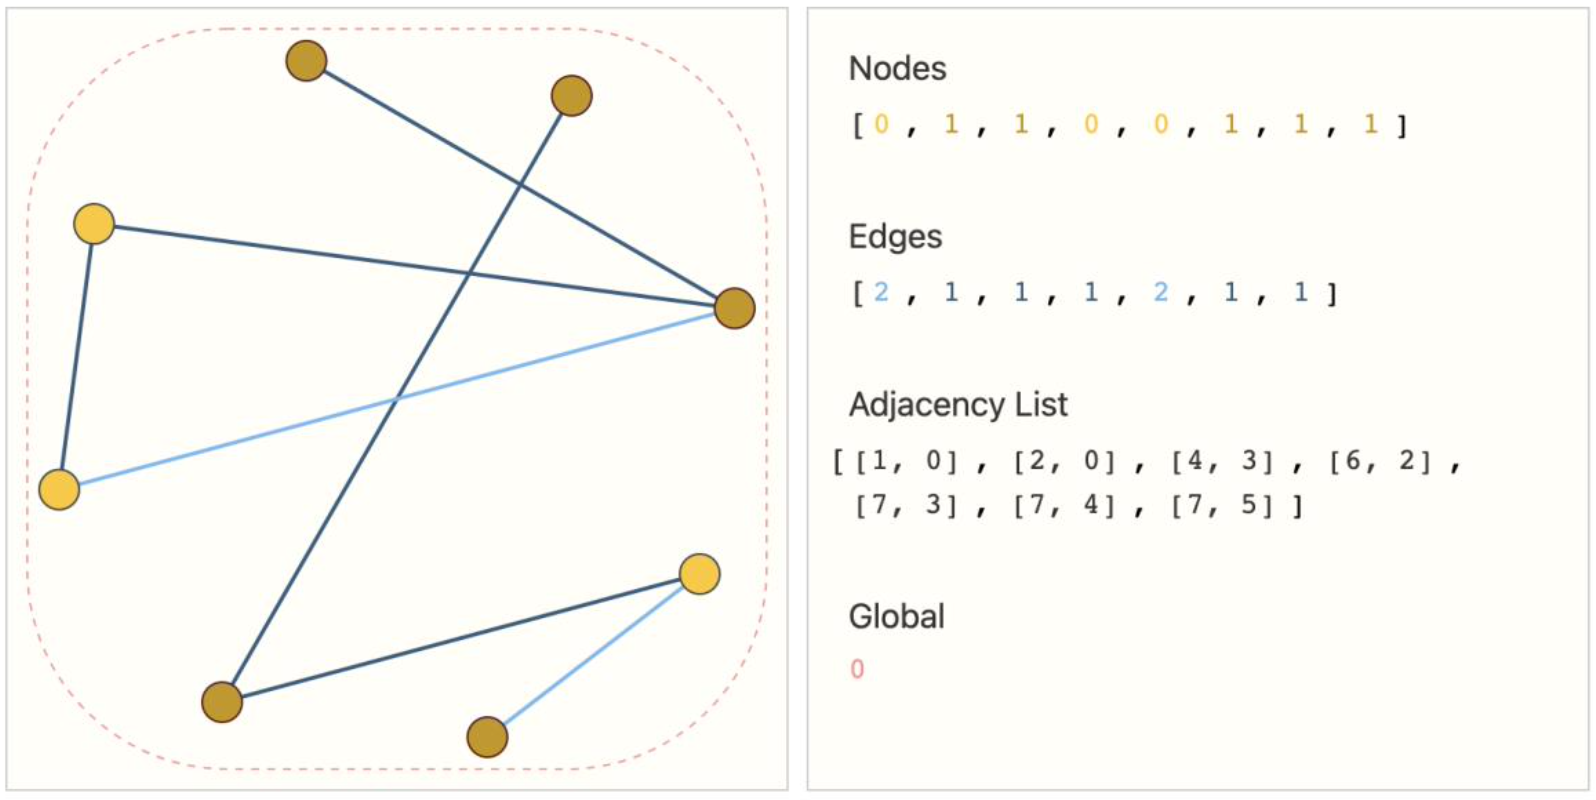
\includegraphics[width=\textwidth]{figure/ComputGraph.png}
    \caption{Rappresentazione tramite lista di adiacenza per un grafo computazionale.}
    \label{fig:GraphComp}
\end{figure}

\section{Graph Neural Network}

Le Graph Neural Network (GNN) sono modelli neurali progettati per apprendere rappresentazioni su strutture a grafo. Una GNN è una trasformazione ottimizzabile che agisce su tutti gli attributi del grafo — nodi, archi e contesto globale — mantenendo invariata la sua struttura topologica (cioè la connettività tra nodi). Nel seguito, descriveremo le GNN seguendo il framework delle Message Passing Neural Network (MPNN), introdotto da Gilmer et al. (2017)~\cite{gilmer2017neural}, e implementato secondo lo schema delle Graph Nets proposte da Battaglia et al. (2018)~\cite{battaglia2018relational}. Questi modelli adottano una filosofia graph-in, graph-out: prendono in input un grafo con attributi associati a nodi, archi e contesto globale, e restituiscono un grafo trasformato, con la stessa struttura ma con rappresentazioni (embedding) aggiornate.

\subsection{La GNN più semplice}

Cominciamo analizzando l’architettura GNN più basilare. In questa configurazione, il modello apprende nuovi embedding per ogni componente del grafo — nodi, archi e contesto globale — senza però sfruttare le relazioni topologiche tra i nodi, cioè senza considerare la connettività. Questa GNN elementare applica un Multilayer Perceptron (MLP) separato a ciascun tipo di elemento del grafo. In particolare, a ogni nodo viene applicata una MLP che restituisce un nuovo embedding; lo stesso avviene per ogni arco e per il vettore del contesto globale. Questo layer viene comunemente definito GNN layer.

\subsection{Pooling delle informazioni}

Il termine pooling nelle GNN fa riferimento all’operazione di aggregazione delle informazioni provenienti da più elementi del grafo (tipicamente nodi o archi), con lo scopo di costruire una rappresentazione compatta dell’intero grafo o di una sua porzione. Questo è particolarmente utile nei compiti di classificazione o regressione a livello di grafo o di sotto-grafo. Nel nostro caso, consideriamo un problema di classificazione binaria a livello di nodo. Se i nodi contengono già informazioni sufficienti, è possibile applicare direttamente una classificazione lineare agli embedding appresi. Tuttavia, non sempre è disponibile informazione utile nei nodi. In queste situazioni, è necessario inferire tali informazioni aggregandole dagli archi adiacenti (Figura~\ref{fig:aggEdg}).
\begin{figure}
    \centering
    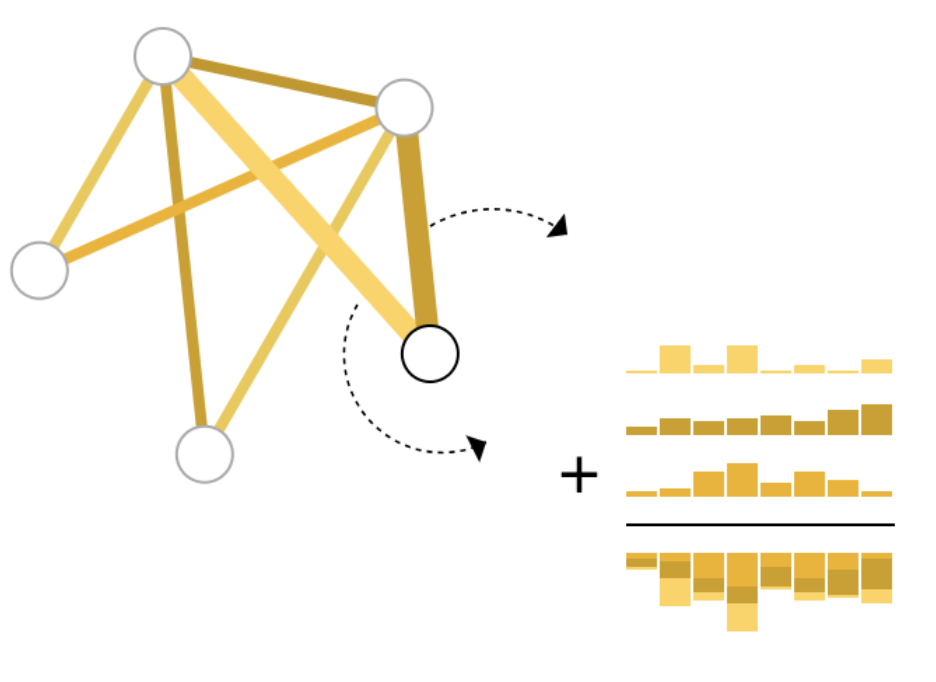
\includegraphics[width=\textwidth]{figure/AggEdges.png}
    \caption{In assenza di informazioni nei nodi, è possibile inferirle aggregando quelle presenti negli archi adiacenti.}
    \label{fig:aggEdg}
\end{figure}
Il processo di pooling può essere formalizzato in due fasi principali:

\begin{enumerate}
    \item Per ciascun elemento da aggregare (es. un nodo), si raccolgono gli embedding degli elementi correlati (es. archi adiacenti), e li si organizza in una matrice.
    \item La matrice ottenuta viene aggregata tramite una funzione, tipicamente una somma o una media, per ottenere un singolo embedding rappresentativo.
\end{enumerate}

Questo approccio, indicato con la funzione $\rho$, è una strategia generica che consente di dedurre informazioni mancanti in un nodo, un arco o nel contesto globale aggregando gli embedding degli elementi circostanti.

\subsection{Message Passing}

Fino a questo punto, l’aggregazione delle informazioni (pooling) è stata eseguita indipendentemente dalla connettività del grafo. Tuttavia, una strategia ben più potente consiste nell’integrare la topologia del grafo nel processo di apprendimento. Questo è possibile grazie alla tecnica del Message Passing. Nel Message Passing, gli elementi del grafo (nodi o archi) scambiano informazioni con i loro vicini, aggiornando i rispettivi embedding in base alla struttura del grafo. Questo meccanismo si articola in tre fasi:

\begin{enumerate}
    \item Per ogni nodo, si raccolgono gli embedding dei nodi adiacenti (e, se necessario, degli archi connessi).
    \item Le informazioni raccolte vengono aggregate tramite una funzione (ad esempio, una somma o una media).
    \item Il risultato dell’aggregazione viene passato a una funzione di aggiornamento (generalmente un MLP) per produrre un nuovo embedding per il nodo.
\end{enumerate}

\begin{figure}
    \centering
    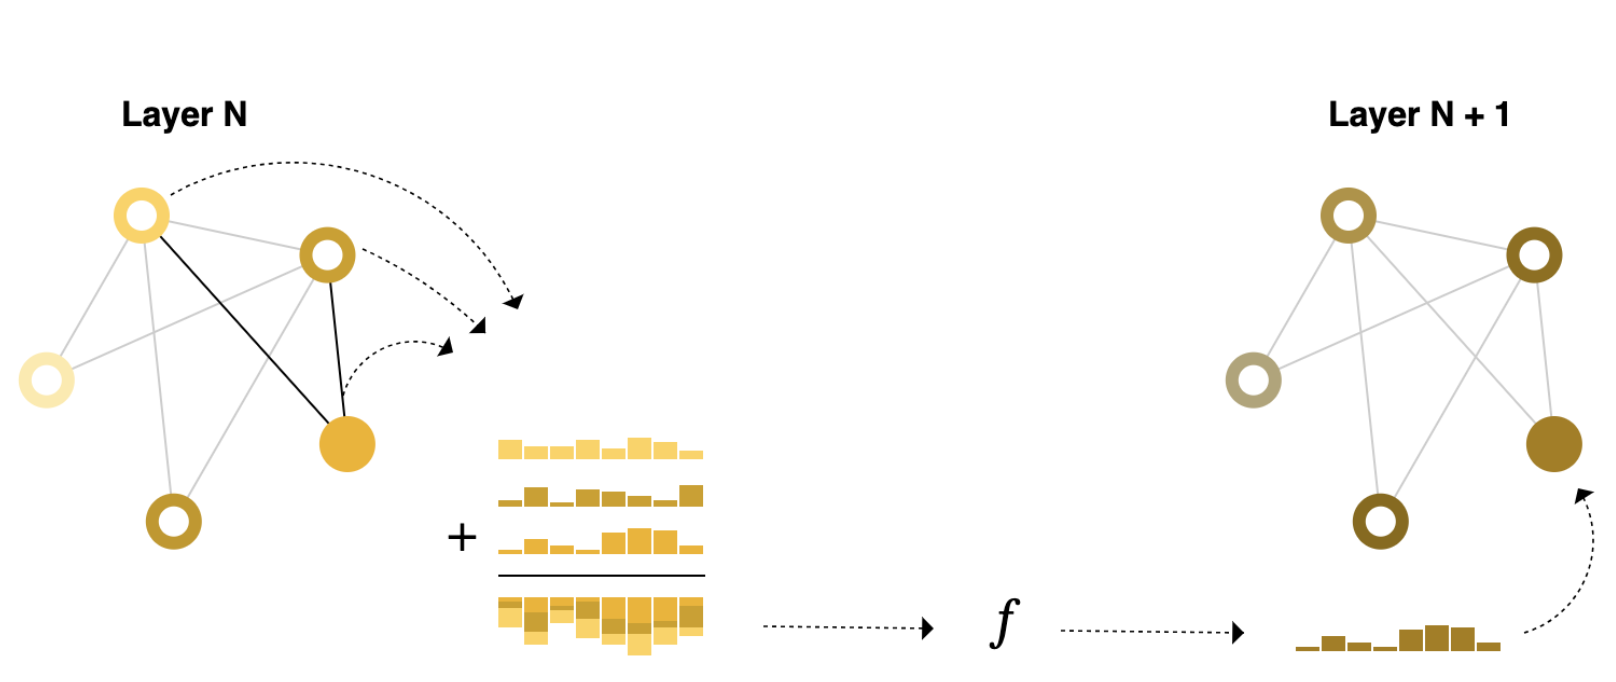
\includegraphics[width=\textwidth]{figure/MessagePassing.png}
    \caption{Fasi della Message Passing: aggregazione dei nodi adiacenti,   trasformazione tramite MLP, aggiornamento degli embedding.}
    \label{fig:messPass}
\end{figure}
Questo processo può essere applicato non solo ai nodi, ma anche agli archi. La grande differenza rispetto, ad esempio, ai pixel in un’immagine, è che i nodi possono trasmettere e ricevere informazioni anche da nodi lontani, potenzialmente aggregando conoscenza da tutto il grafo. Un ulteriore miglioramento consiste nel far avvenire la condivisione delle informazioni già durante il processo di message passing, anziché solo al termine. Tuttavia, combinare direttamente embedding di nodi e archi può non essere immediato, poiché questi vettori possono avere dimensioni diverse. Una soluzione comune è apprendere mappature lineari tra lo spazio degli archi e quello dei nodi (e viceversa), per permettere una corretta integrazione delle informazioni. La scelta della sequenza e del tipo di aggiornamenti rappresenta un'importante decisione di progettazione dell'architettura GNN.

\subsection{Rappresentazione globale}

Una delle limitazioni delle reti descritte finora risiede nella difficoltà di trasferire efficacemente informazioni tra nodi molto distanti all’interno del grafo. Anche applicando la tecnica del message passing in maniera ripetuta, le informazioni potrebbero non propagarsi in modo efficiente. Una possibile soluzione consisterebbe nel consentire a ogni nodo di comunicare direttamente con tutti gli altri; tuttavia, questa strategia risulterebbe computazionalmente onerosa. Una soluzione alternativa, più efficiente, è quella di fornire a ciascun nodo una \textbf{rappresentazione globale}, solitamente indicata con $U$, nota anche come \textbf{Master Node}. Questo contesto globale è connesso a tutti i nodi e archi del grafo, e agisce come un canale condiviso per lo scambio di informazioni tra le componenti del grafo. Tale approccio consente di costruire una rappresentazione più ricca e articolata dell’intero grafo, che può essere appresa durante l’addestramento.

\subsubsection{Conditioning}

Un metodo efficace per arricchire l'embedding di un nodo consiste nel \textbf{conditionig}, che prevede l'integrazione delle informazioni locali con quelle provenienti dai nodi e dagli archi adiacenti, oltre al contesto globale. Questa tecnica porta alla costruzione di rappresentazioni più informative e robuste (Figura~\ref{fig:condit}).

\begin{figure}
    \centering
    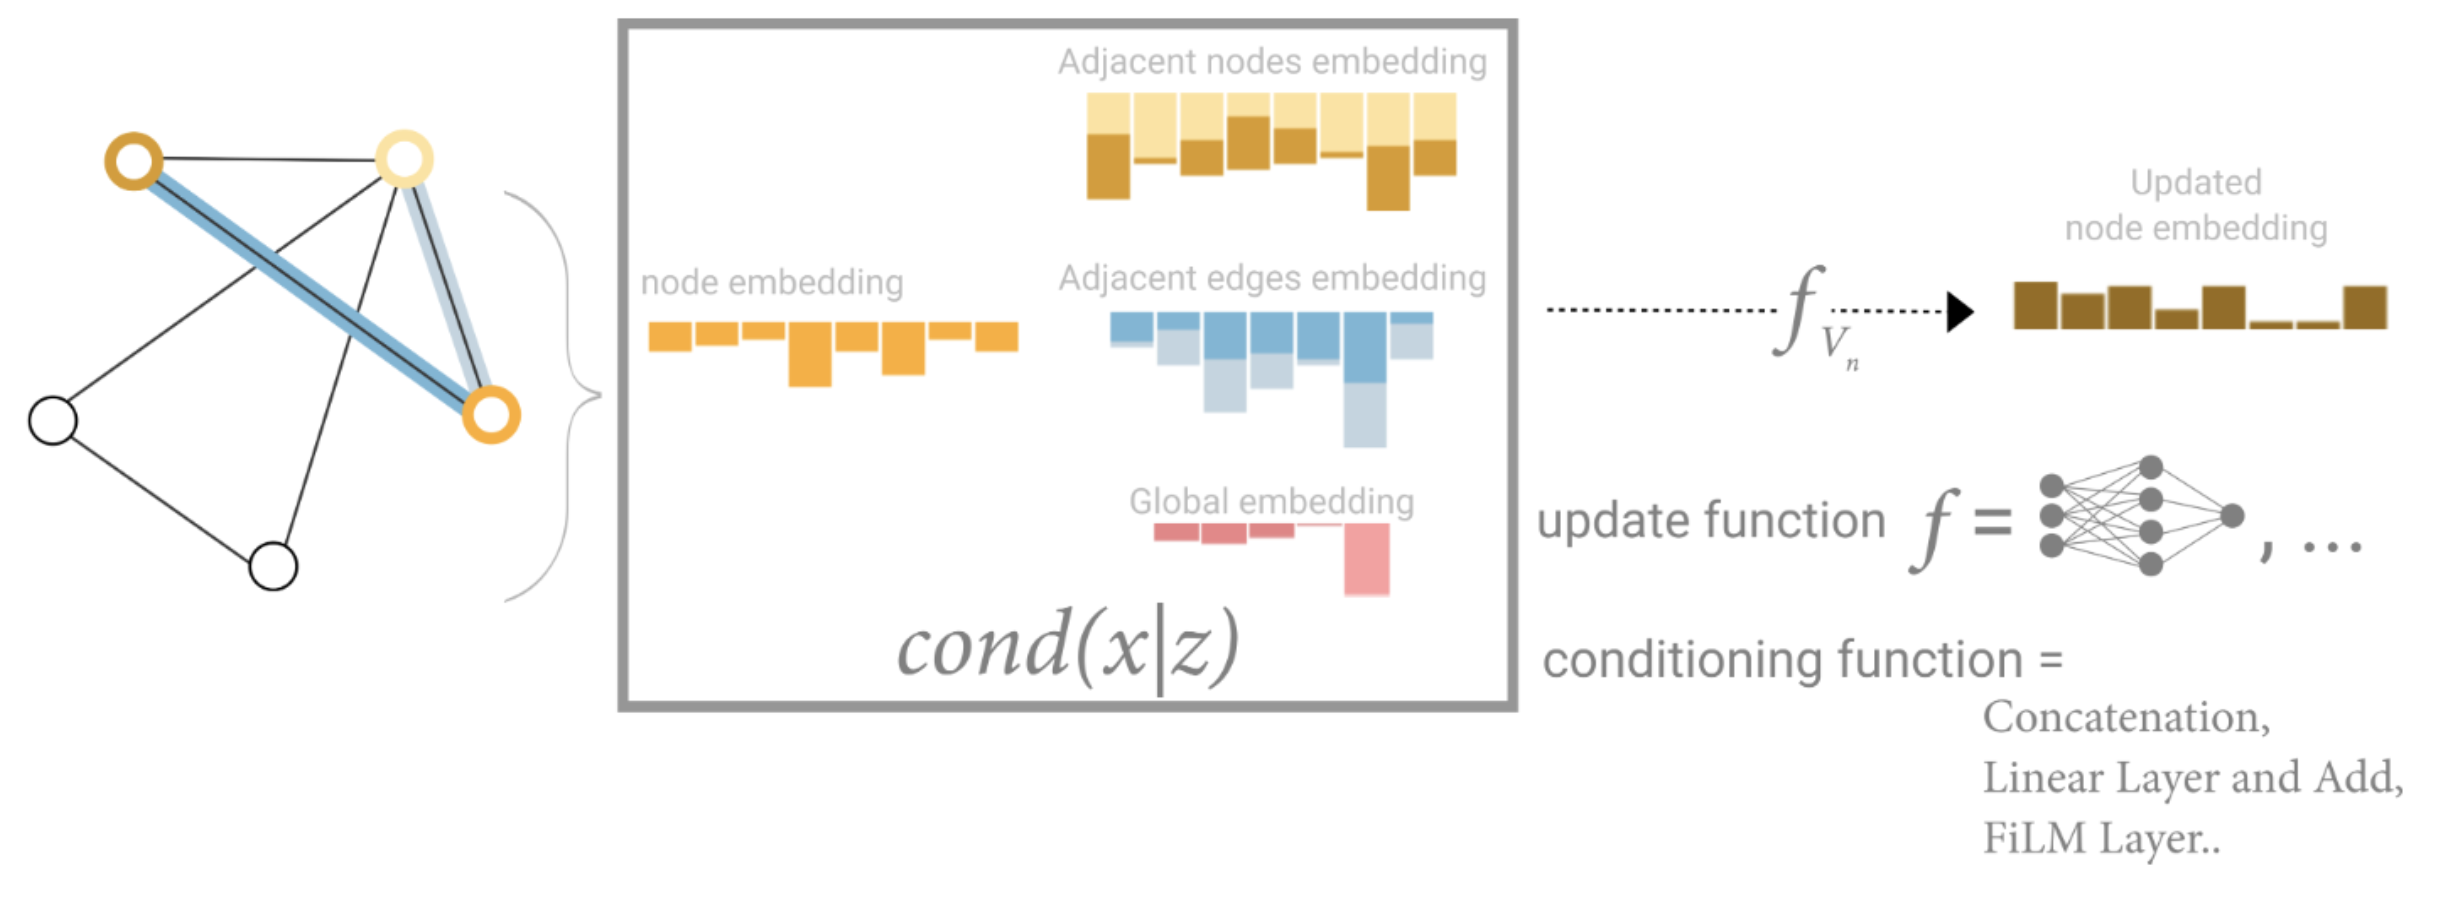
\includegraphics[width=\textwidth]{figure/Conditioning.png}
    \caption{Rappresentazione del Conditioning applicato all'embedding di un nodo, arricchito mediante gli embedding dei nodi e degli archi adiacenti, e quello relativo al contesto globale.}
    \label{fig:condit}
\end{figure}

\subsection{Filtri polinomiali sui grafi}

Nelle Graph Neural Networks (GNN), i \textit{filtri polinomiali} rappresentano uno strumento chiave per estendere il concetto di convoluzione ai dati strutturati sotto forma di grafo. In questa sezione ne descriviamo la formulazione, l’interpretazione e i vantaggi.

\subsubsection{Il Laplaciano del grafo}

Dato un grafo \( G = (V, E) \) con matrice di adiacenza \( A \), la \textbf{matrice dei gradi} \( D \) è definita come:
\[
  D_{ii} = \sum_{j} A_{ij}
\]
Il \textbf{Laplaciano non normalizzato} del grafo è dato da:
\[
  L = D - A
\]
Una versione alternativa è il \textbf{Laplaciano normalizzato}:
\[
  \mathcal{L} = I - D^{-1/2} A D^{-1/2}
\]
Tale operatore discreto è l’analogo del Laplaciano continuo impiegato in analisi matematica e fisica. Definito \( L \), è possibile costruire polinomi in \( L \):
\[
  p_w(L) = \sum_{k=0}^d w_k L^k
\]
dove:
\begin{itemize}
  \item \( w_k \) sono coefficienti (parametri appresi);
  \item \( d \) è il grado del polinomio.
\end{itemize}
L’operazione \( p_w(L) x \) consente di propagare le feature \( x \in \mathbb{R}^n \) tra nodi a distanza crescente.

\subsubsection{Interpretazione: Convoluzione Locale}

Ogni potenza \( L^k \) consente di aggregare informazioni da nodi situati entro \( k \) hop nel grafo:
\begin{itemize}
  \item \( L^0 x = x \): solo il nodo corrente;
  \item \( Lx \): include i vicini diretti;
  \item \( L^2 x \): considera anche i vicini dei vicini.
\end{itemize}
Il filtro \( p_w(L) \) si comporta quindi come un kernel convoluzionale con raggio \( d \).

\subsubsection{Esempio: Filtro di grado 1}
Consideriamo il filtro:
\[
  p_w(L) = w_0 I + w_1 L
\]
Applicandolo a un vettore \( x \), otteniamo:
\[
  x' = w_0 x + w_1 Lx
\]
Questa è l’idea alla base della GCN classica.

\subsection{Chebyshev Polynomials (ChebNet)}

\textbf{ChebNet} rappresenta un’evoluzione dei filtri polinomiali, utilizzando i \textbf{polinomi di Chebyshev} \( T_k(x) \), definiti ricorsivamente:
\[
\begin{aligned}
  T_0(x) &= 1 \\
  T_1(x) &= x \\
  T_{k+1}(x) &= 2x T_k(x) - T_{k-1}(x)
\end{aligned}
\]
Il filtro convoluzionale in ChebNet è:
\[
  x' = \sum_{k=0}^K w_k T_k(\tilde{L}) x
\]
dove \( \tilde{L} = \frac{2L}{\lambda_{\text{max}}(L)} - I \) è una versione normalizzata del Laplaciano, i cui autovalori sono in \([-1, 1]\).

\subsubsection{Vantaggi dei polinomi di Chebyshev}

\begin{itemize}
  \item Maggiore stabilità numerica grazie al dominio limitato \([-1, 1]\);
  \item Convoluzioni localizzate computazionalmente efficienti;
  \item Equivarianza rispetto all’ordine dei nodi (i risultati si trasformano coerentemente sotto permutazioni dei nodi).
\end{itemize}

\subsubsection{Stacking e Non-linearità}

Analogamente alle CNN, i filtri possono essere:
\begin{itemize}
  \item Impilati in più layer;
  \item Seguiti da funzioni non lineari (es. ReLU).
\end{itemize}
Questo consente l’apprendimento di rappresentazioni gerarchiche sempre più complesse.

\subsection{GNN in breve}

Una GNN esegue il processo di \textit{message passing} in modo iterativo tra i layer. La forma generale è:

\begin{enumerate}
    \item \textbf{Aggregazione}: per ogni nodo \( i \):
    \[
        m_i^{(l)} = \sum_{j\in \mathcal{N}(i)} f^{(l)}(h_j^{(l-1)}, h_i^{(l-1)}, e_{ij})
    \]
    dove \( h_j^{(l-1)} \) e \( h_i^{(l-1)} \) sono gli embedding al livello precedente, ed \( e_{ij} \) rappresenta le feature dell’arco.
    \item \textbf{Aggiornamento}:
    \[
        h_i^{(l)} = g^{(l)}(h_i^{(l-1)}, m_i^{(l)})
    \]
    dove \( g \) è una funzione appresa.
    \item \textbf{Readout}: una funzione aggrega le rappresentazioni dei nodi per ottenere quella dell’intero grafo.
\end{enumerate}

\section{Modern Graph Neural Networks}

Cosa accade se, invece di filtri polinomiali, adottiamo strategie di aggregazione alternative? È importante che l’aggregazione sia invariante all’ordine dei nodi, così da garantire robustezza strutturale. In questi modelli, la convoluzione viene vista come un processo di message passing iterato. Ogni nodo aggiorna la propria rappresentazione combinando la propria feature con quelle dei nodi adiacenti.

\subsection{Graph Convolutional Network (GCN)}

Una GCN segue due step fondamentali:
\begin{enumerate}
    \item \textbf{Aggregazione} delle feature dai vicini:
    \[
        h_v^{(k)} = f^{(k)}\left(W^{(k)} \cdot \frac{1}{|\mathcal{N}(v)|} \sum_{u \in \mathcal{N}(v)} h_u^{(k-1)} + B^{(k)} \cdot h_v^{(k-1)}\right)
    \]
    \item \textbf{Predizione} finale:
    \[
        \hat y_v = \operatorname{PREDICT}(h_v^{(K)})
    \]
\end{enumerate}

La funzione \( \operatorname{PREDICT} \) è una rete neurale addestrata congiuntamente al modello GCN. Le matrici \( W^{(k)} \) e \( B^{(k)} \) sono condivise tra i nodi e non dipendono dalla dimensione del grafo, il che rende il modello scalabile.

\subsection{GCN in breve}

La GCN è una GNN che utilizza convoluzioni su grafi. Per ogni layer:
\begin{enumerate}
    \item \textbf{Aggregazione normalizzata}:
    \[
        m_i^{(l)} = \sum_{j\in \mathcal{N}(i)} \frac{1}{\sqrt{d_i d_j}} h_j^{(l-1)}
    \]
    \item \textbf{Aggiornamento non lineare}:
    \[
        h_i^{(l)} = \sigma(W^{(l)} m_i^{(l)})
    \]
\end{enumerate}

\textbf{Conclusione:} GNN è un termine generico, mentre GCN è un’architettura specifica che applica convoluzioni sui grafi tramite aggregazione e trasformazioni lineari.

\subsection{Graph Attention Network (GAT)}

La GAT introduce un meccanismo di attenzione:
\[
    h_v^{(k)} = f^{(k)}\left(W^{(k)} \cdot \sum_{u \in \mathcal{N}(v)} \alpha_{vu}^{(k-1)} h_u^{(k-1)} + \alpha_{vv}^{(k-1)} h_v^{(k-1)}\right)
\]
dove i pesi di attenzione sono definiti come:
\[
    \alpha_{vu}^{(k)} = \frac{A^{(k)}(h_v^{(k)}, h_u^{(k)})}{\sum_{w\in\mathcal{N}(v)} A^{(k)}(h_v^{(k)}, h_w^{(k)})}
\]
Infine:
\[
    \hat y_v = \operatorname{PREDICT}(h_v^{(K)})
\]
I parametri \( f, W, A \) sono condivisi tra i nodi. Questo rende la GAT efficiente e scalabile.

\subsection{Graph SAGE}

\textbf{Graph SAGE} (Graph Sample and AggregatE) è un'architettura di GNN proposta per affrontare il problema della generalizzazione a nodi non visti durante il training, ovvero il cosiddetto \textit{inductive setting}. Invece di apprendere una rappresentazione per ogni nodo del grafo (come avviene nei metodi trasduttivi), Graph SAGE apprende una funzione di aggregazione che può essere applicata anche a nodi mai visti. Il principio di base è quello di aggiornare le rappresentazioni dei nodi tramite l'aggregazione delle feature dei vicini campionati:
\[
    h_v^{(k)} = \sigma\left(W^{(k)} \cdot \text{AGGREGATE}^{(k)}\left(\{h_v^{(k-1)}\} \cup \{h_u^{(k-1)}, \forall u \in \mathcal{N}(v)\}\right)\right)
\]
Dove:
\begin{itemize}
    \item \( h_v^{(k)} \) rappresenta l'embedding del nodo \( v \) al layer \( k \),
    \item \( \mathcal{N}(v) \) è l'insieme dei vicini di \( v \),
    \item \( \text{AGGREGATE}^{(k)} \) è una funzione (non parametrica o parametrica) che aggrega le rappresentazioni dei vicini,
    \item \( W^{(k)} \) è una matrice di pesi appresa,
    \item \( \sigma \) è una funzione di attivazione non lineare (es. ReLU).
\end{itemize}

Alcune possibili scelte per la funzione di aggregazione includono:
\begin{itemize}
    \item \texttt{mean}: media delle rappresentazioni dei vicini,
    \item \texttt{pooling}: max- o mean-pooling dopo un MLP,
    \item \texttt{LSTM}: aggregazione sequenziale tramite un LSTM.
\end{itemize}

L’approccio di Graph SAGE è particolarmente utile per scenari di \textit{streaming} o \textit{large-scale learning}, poiché permette di scalare a grafi di grandi dimensioni grazie al campionamento locale e al riutilizzo della stessa funzione aggregatrice.

\subsection{GIN}

La \textbf{Graph Isomorphism Network} (GIN) è un'architettura proposta con l’obiettivo di massimizzare il potere discriminante delle GNN. In particolare, GIN si basa sull’intuizione che molte architetture GNN esistenti non riescono a distinguere efficacemente tra strutture topologicamente diverse. GIN è costruita in modo da essere potente quanto il test di isomorfismo di Weisfeiler-Lehman (WL test), noto per la sua efficacia nel distinguere grafi non isomorfi. La formula di aggiornamento per un nodo \( v \) è la seguente:
\[
    h_v^{(k)} = \text{MLP}^{(k)} \left((1 + \epsilon^{(k)}) \cdot h_v^{(k-1)} + \sum_{u \in \mathcal{N}(v)} h_u^{(k-1)} \right)
\]
Dove:
\begin{itemize}
    \item \( \epsilon^{(k)} \) è un parametro (appreso o fisso) che bilancia il contributo del nodo rispetto ai suoi vicini,
    \item \( \text{MLP}^{(k)} \) è un multilayer perceptron che apprende una trasformazione non lineare,
    \item \( h_v^{(k)} \) rappresenta l’embedding del nodo al layer \( k \).
\end{itemize}

GIN evita normalizzazioni e pesi di attenzione, puntando su un'aggregazione semplice ma espressiva, dove l'intera struttura locale del nodo viene catturata sommando direttamente le rappresentazioni. È stato dimostrato empiricamente che GIN ottiene prestazioni molto competitive su compiti di classificazione di grafi e predizione sui nodi, grazie alla sua capacità di distinguere strutture complesse.

\begin{sidewaystable}[htbp]
    \centering
    \caption{Confronto tra le principali architetture di Graph Neural Networks.}
    \scriptsize
    \begin{tabular}{|l|c|c|c|c|}
    \hline
    \textbf{Caratteristica} & \textbf{GCN} & \textbf{GAT} & \textbf{GraphSAGE} & \textbf{GIN} \\
    \hline
    \textbf{Tipo Aggregazione} & Media normalizzata & Attenzione pesata & Custom (media, LSTM, pooling) & Somma + MLP \\
    \hline
    \textbf{Pesatura dei vicini} & Statica (matrice normalizzata) & Dinamica (self-attention) & Parametrica o fissa & Fissa (somma) \\
    \hline
    \textbf{Apprendimento Induttivo} & No & Parziale & Sì & No \\
    \hline
    \textbf{Espressività} & Limitata & Superiore a GCN & Dipende dall’aggregatore & Massima (WL test) \\
    \hline
    \textbf{Funzione di aggiornamento} & Lineare + ReLU & Lineare + Attenzione & MLP + Aggregazione & MLP su somma \\
    \hline
    \textbf{Parametri appresi} & W & W, Attenzione & W, Aggregatore (opz.) & MLP, $\epsilon$ \\
    \hline
    \textbf{Sensibile alla struttura del grafo} & Sì & Sì & Sì & Sì (con maggiore discriminatività) \\
    \hline
    \textbf{Scalabilità} & Buona & Limitata (per grafi molto grandi) & Alta (con campionamento) & Media \\
    \hline
    \textbf{Proprietà chiave} & Semplicità & Flessibilità & Generalizzazione & Massima capacità discriminante \\
    \hline
    \end{tabular}
\label{tab:GNN_comparison}
\end{sidewaystable}

